\documentclass[twoside]{book}

% Packages required by doxygen
\usepackage{fixltx2e}
\usepackage{calc}
\usepackage{doxygen}
\usepackage[export]{adjustbox} % also loads graphicx
\usepackage{graphicx}
\usepackage[utf8]{inputenc}
\usepackage{makeidx}
\usepackage{multicol}
\usepackage{multirow}
\PassOptionsToPackage{warn}{textcomp}
\usepackage{textcomp}
\usepackage[nointegrals]{wasysym}
\usepackage[table]{xcolor}

% Font selection
\usepackage[T1]{fontenc}
\usepackage[scaled=.90]{helvet}
\usepackage{courier}
\usepackage{amssymb}
\usepackage{sectsty}
\renewcommand{\familydefault}{\sfdefault}
\allsectionsfont{%
  \fontseries{bc}\selectfont%
  \color{darkgray}%
}
\renewcommand{\DoxyLabelFont}{%
  \fontseries{bc}\selectfont%
  \color{darkgray}%
}
\newcommand{\+}{\discretionary{\mbox{\scriptsize$\hookleftarrow$}}{}{}}

% Page & text layout
\usepackage{geometry}
\geometry{%
  a4paper,%
  top=2.5cm,%
  bottom=2.5cm,%
  left=2.5cm,%
  right=2.5cm%
}
\tolerance=750
\hfuzz=15pt
\hbadness=750
\setlength{\emergencystretch}{15pt}
\setlength{\parindent}{0cm}
\setlength{\parskip}{0.2cm}
\makeatletter
\renewcommand{\paragraph}{%
  \@startsection{paragraph}{4}{0ex}{-1.0ex}{1.0ex}{%
    \normalfont\normalsize\bfseries\SS@parafont%
  }%
}
\renewcommand{\subparagraph}{%
  \@startsection{subparagraph}{5}{0ex}{-1.0ex}{1.0ex}{%
    \normalfont\normalsize\bfseries\SS@subparafont%
  }%
}
\makeatother

% Headers & footers
\usepackage{fancyhdr}
\pagestyle{fancyplain}
\fancyhead[LE]{\fancyplain{}{\bfseries\thepage}}
\fancyhead[CE]{\fancyplain{}{}}
\fancyhead[RE]{\fancyplain{}{\bfseries\leftmark}}
\fancyhead[LO]{\fancyplain{}{\bfseries\rightmark}}
\fancyhead[CO]{\fancyplain{}{}}
\fancyhead[RO]{\fancyplain{}{\bfseries\thepage}}
\fancyfoot[LE]{\fancyplain{}{}}
\fancyfoot[CE]{\fancyplain{}{}}
\fancyfoot[RE]{\fancyplain{}{\bfseries\scriptsize Generated on Sat Jul 8 2017 14\+:20\+:04 for T\+P2 trab 3 by Doxygen }}
\fancyfoot[LO]{\fancyplain{}{\bfseries\scriptsize Generated on Sat Jul 8 2017 14\+:20\+:04 for T\+P2 trab 3 by Doxygen }}
\fancyfoot[CO]{\fancyplain{}{}}
\fancyfoot[RO]{\fancyplain{}{}}
\renewcommand{\footrulewidth}{0.4pt}
\renewcommand{\chaptermark}[1]{%
  \markboth{#1}{}%
}
\renewcommand{\sectionmark}[1]{%
  \markright{\thesection\ #1}%
}

% Indices & bibliography
\usepackage{natbib}
\usepackage[titles]{tocloft}
\setcounter{tocdepth}{3}
\setcounter{secnumdepth}{5}
\makeindex

% Hyperlinks (required, but should be loaded last)
\usepackage{ifpdf}
\ifpdf
  \usepackage[pdftex,pagebackref=true]{hyperref}
\else
  \usepackage[ps2pdf,pagebackref=true]{hyperref}
\fi
\hypersetup{%
  colorlinks=true,%
  linkcolor=blue,%
  citecolor=blue,%
  unicode%
}

% Custom commands
\newcommand{\clearemptydoublepage}{%
  \newpage{\pagestyle{empty}\cleardoublepage}%
}


%===== C O N T E N T S =====

\begin{document}

% Titlepage & ToC
\hypersetup{pageanchor=false,
             bookmarks=true,
             bookmarksnumbered=true,
             pdfencoding=unicode
            }
\pagenumbering{roman}
\begin{titlepage}
\vspace*{7cm}
\begin{center}%
{\Large T\+P2 trab 3 }\\
\vspace*{1cm}
{\large Generated by Doxygen 1.8.9.1}\\
\vspace*{0.5cm}
{\small Sat Jul 8 2017 14:20:04}\\
\end{center}
\end{titlepage}
\clearemptydoublepage
\tableofcontents
\clearemptydoublepage
\pagenumbering{arabic}
\hypersetup{pageanchor=true}

%--- Begin generated contents ---
\chapter{File Index}
\section{File List}
Here is a list of all files with brief descriptions\+:\begin{DoxyCompactList}
\item\contentsline{section}{\hyperlink{controllers_8cpp}{controllers.\+cpp} }{\pageref{controllers_8cpp}}{}
\item\contentsline{section}{\hyperlink{controllers_8hpp}{controllers.\+hpp} }{\pageref{controllers_8hpp}}{}
\item\contentsline{section}{\hyperlink{helper_8cpp}{helper.\+cpp} }{\pageref{helper_8cpp}}{}
\item\contentsline{section}{\hyperlink{helper_8hpp}{helper.\+hpp} }{\pageref{helper_8hpp}}{}
\item\contentsline{section}{\hyperlink{interfaces_8hpp}{interfaces.\+hpp} }{\pageref{interfaces_8hpp}}{}
\item\contentsline{section}{\hyperlink{main_8cpp}{main.\+cpp} }{\pageref{main_8cpp}}{}
\item\contentsline{section}{\hyperlink{question_8cpp}{question.\+cpp} }{\pageref{question_8cpp}}{}
\item\contentsline{section}{\hyperlink{question_8hpp}{question.\+hpp} }{\pageref{question_8hpp}}{}
\item\contentsline{section}{\hyperlink{quiz_8cpp}{quiz.\+cpp} }{\pageref{quiz_8cpp}}{}
\item\contentsline{section}{\hyperlink{quiz_8hpp}{quiz.\+hpp} }{\pageref{quiz_8hpp}}{}
\item\contentsline{section}{\hyperlink{stub_p_r_8cpp}{stub\+P\+R.\+cpp} }{\pageref{stub_p_r_8cpp}}{}
\item\contentsline{section}{\hyperlink{stub_p_r_8hpp}{stub\+P\+R.\+hpp} }{\pageref{stub_p_r_8hpp}}{}
\item\contentsline{section}{\hyperlink{subject_8cpp}{subject.\+cpp} }{\pageref{subject_8cpp}}{}
\item\contentsline{section}{\hyperlink{subject_8hpp}{subject.\+hpp} }{\pageref{subject_8hpp}}{}
\item\contentsline{section}{\hyperlink{topic_8cpp}{topic.\+cpp} }{\pageref{topic_8cpp}}{}
\item\contentsline{section}{\hyperlink{topic_8hpp}{topic.\+hpp} }{\pageref{topic_8hpp}}{}
\item\contentsline{section}{\hyperlink{user_8cpp}{user.\+cpp} }{\pageref{user_8cpp}}{}
\item\contentsline{section}{\hyperlink{user_8hpp}{user.\+hpp} }{\pageref{user_8hpp}}{}
\end{DoxyCompactList}

\chapter{File Documentation}
\hypertarget{controllers_8cpp}{}\section{controllers.\+cpp File Reference}
\label{controllers_8cpp}\index{controllers.\+cpp@{controllers.\+cpp}}
{\ttfamily \#include $<$cstdio$>$}\newline
{\ttfamily \#include $<$iostream$>$}\newline
{\ttfamily \#include $<$string$>$}\newline
{\ttfamily \#include $<$typeinfo$>$}\newline
{\ttfamily \#include $<$map$>$}\newline
{\ttfamily \#include $<$algorithm$>$}\newline
{\ttfamily \#include \char`\"{}user.\+hpp\char`\"{}}\newline
{\ttfamily \#include \char`\"{}controllers.\+hpp\char`\"{}}\newline
{\ttfamily \#include \char`\"{}stub\+P\+R.\+hpp\char`\"{}}\newline

\hypertarget{helper_8cpp}{}\section{helper.\+cpp File Reference}
\label{helper_8cpp}\index{helper.\+cpp@{helper.\+cpp}}
{\ttfamily \#include \char`\"{}helper.\+hpp\char`\"{}}\newline
{\ttfamily \#include $<$list$>$}\newline
{\ttfamily \#include $<$cstdlib$>$}\newline
{\ttfamily \#include $<$ctime$>$}\newline
{\ttfamily \#include $<$cstdio$>$}\newline
{\ttfamily \#include $<$algorithm$>$}\newline
\subsection*{Functions}
\begin{DoxyCompactItemize}
\item 
std\+::vector$<$ int $>$ \hyperlink{helper_8cpp_aff8265ecd56d0f933b5d78cefd93ff32}{randompermutation} (int size)
\begin{DoxyCompactList}\small\item\em /$\ast$ \end{DoxyCompactList}\item 
std\+::queue$<$ int $>$ \hyperlink{helper_8cpp_a0bbe636bfe707cc196c9eadbca4416c7}{randompermutationQ} (int size)
\item 
int \hyperlink{helper_8cpp_a4d580e96dfaa8723fedadc161627fac1}{read\+Int\+In\+Range} (int L, int R)
\begin{DoxyCompactList}\small\item\em Fun��o para verificar se um inteiro lido do teclado est� em um range (intervalo) v�lido. \end{DoxyCompactList}\item 
bool \hyperlink{helper_8cpp_a056f915ac39307039d2855e9afd1dcf2}{is\+Alpha\+Numerical} (char c)
\begin{DoxyCompactList}\small\item\em Fun��o para verificar se um caractere lido do teclado � alfanum�rico, usando a tabela A\+S\+C\+II. \end{DoxyCompactList}\item 
char \hyperlink{helper_8cpp_a831a2329c820ba9b9b378131ed143ff5}{readchar} ()
\begin{DoxyCompactList}\small\item\em Fun�ao que le um caractere ret do teclado enquanto o caractere ret lido n�o � alfanumerico. \end{DoxyCompactList}\end{DoxyCompactItemize}


\subsection{Function Documentation}
\mbox{\Hypertarget{helper_8cpp_a056f915ac39307039d2855e9afd1dcf2}\label{helper_8cpp_a056f915ac39307039d2855e9afd1dcf2}} 
\index{helper.\+cpp@{helper.\+cpp}!is\+Alpha\+Numerical@{is\+Alpha\+Numerical}}
\index{is\+Alpha\+Numerical@{is\+Alpha\+Numerical}!helper.\+cpp@{helper.\+cpp}}
\subsubsection{\texorpdfstring{is\+Alpha\+Numerical()}{isAlphaNumerical()}}
{\footnotesize\ttfamily bool is\+Alpha\+Numerical (\begin{DoxyParamCaption}\item[{char}]{ }\end{DoxyParamCaption})}



Fun��o para verificar se um caractere lido do teclado � alfanum�rico, usando a tabela A\+S\+C\+II. 


\begin{DoxyParams}{Parameters}
{\em um} & char. \\
\hline
\end{DoxyParams}
\begin{DoxyReturn}{Returns}
um booleano indicando se o caractere � alfanum�rico ou n�o. 
\end{DoxyReturn}


Definition at line 38 of file helper.\+cpp.

\mbox{\Hypertarget{helper_8cpp_aff8265ecd56d0f933b5d78cefd93ff32}\label{helper_8cpp_aff8265ecd56d0f933b5d78cefd93ff32}} 
\index{helper.\+cpp@{helper.\+cpp}!randompermutation@{randompermutation}}
\index{randompermutation@{randompermutation}!helper.\+cpp@{helper.\+cpp}}
\subsubsection{\texorpdfstring{randompermutation()}{randompermutation()}}
{\footnotesize\ttfamily std\+::vector$<$int$>$ randompermutation (\begin{DoxyParamCaption}\item[{int}]{size }\end{DoxyParamCaption})}



/$\ast$ 

Arquivo contendo funcoes que servem de auxilio para \hyperlink{topic_8cpp}{topic.\+cpp}, \hyperlink{subject_8cpp}{subject.\+cpp}, \hyperlink{user_8cpp}{user.\+cpp}, \hyperlink{helper_8cpp}{helper.\+cpp}, \hyperlink{controllers_8cpp}{controllers.\+cpp}.

\begin{DoxyAuthor}{Author}
joseleite19 
\end{DoxyAuthor}
\begin{DoxySince}{Since}
07/05/2017 
\end{DoxySince}
\begin{DoxyVersion}{Version}
3.\+0 
\end{DoxyVersion}


Definition at line 16 of file helper.\+cpp.

\mbox{\Hypertarget{helper_8cpp_a0bbe636bfe707cc196c9eadbca4416c7}\label{helper_8cpp_a0bbe636bfe707cc196c9eadbca4416c7}} 
\index{helper.\+cpp@{helper.\+cpp}!randompermutationQ@{randompermutationQ}}
\index{randompermutationQ@{randompermutationQ}!helper.\+cpp@{helper.\+cpp}}
\subsubsection{\texorpdfstring{randompermutation\+Q()}{randompermutationQ()}}
{\footnotesize\ttfamily std\+::queue$<$int$>$ randompermutationQ (\begin{DoxyParamCaption}\item[{int}]{size }\end{DoxyParamCaption})}



Definition at line 22 of file helper.\+cpp.

\mbox{\Hypertarget{helper_8cpp_a831a2329c820ba9b9b378131ed143ff5}\label{helper_8cpp_a831a2329c820ba9b9b378131ed143ff5}} 
\index{helper.\+cpp@{helper.\+cpp}!readchar@{readchar}}
\index{readchar@{readchar}!helper.\+cpp@{helper.\+cpp}}
\subsubsection{\texorpdfstring{readchar()}{readchar()}}
{\footnotesize\ttfamily char readchar (\begin{DoxyParamCaption}{ }\end{DoxyParamCaption})}



Fun�ao que le um caractere ret do teclado enquanto o caractere ret lido n�o � alfanumerico. 


\begin{DoxyParams}{Parameters}
{\em n�o} & h�. \\
\hline
\end{DoxyParams}
\begin{DoxySeeAlso}{See also}
\hyperlink{helper_8hpp_a2a6ec05797a0335af4c07553282cc302}{is\+Alpha\+Numerical()} 
\end{DoxySeeAlso}
\begin{DoxyReturn}{Returns}
o caractere ret. 
\end{DoxyReturn}


Definition at line 43 of file helper.\+cpp.

\mbox{\Hypertarget{helper_8cpp_a4d580e96dfaa8723fedadc161627fac1}\label{helper_8cpp_a4d580e96dfaa8723fedadc161627fac1}} 
\index{helper.\+cpp@{helper.\+cpp}!read\+Int\+In\+Range@{read\+Int\+In\+Range}}
\index{read\+Int\+In\+Range@{read\+Int\+In\+Range}!helper.\+cpp@{helper.\+cpp}}
\subsubsection{\texorpdfstring{read\+Int\+In\+Range()}{readIntInRange()}}
{\footnotesize\ttfamily int read\+Int\+In\+Range (\begin{DoxyParamCaption}\item[{int}]{,  }\item[{int}]{ }\end{DoxyParamCaption})}



Fun��o para verificar se um inteiro lido do teclado est� em um range (intervalo) v�lido. 

Ser� lido do teclado o inteiro e depois vamos continuar lendo at� que o inteiro esteja no range v�lido. 
\begin{DoxyParams}{Parameters}
{\em um} & inteiro L e R que representa o range. \\
\hline
\end{DoxyParams}
\begin{DoxyReturn}{Returns}
um inteiro. 
\end{DoxyReturn}


Definition at line 28 of file helper.\+cpp.


\hypertarget{main_8cpp}{}\section{main.\+cpp File Reference}
\label{main_8cpp}\index{main.\+cpp@{main.\+cpp}}
{\ttfamily \#include \char`\"{}controllers.\+hpp\char`\"{}}\newline
\subsection*{Functions}
\begin{DoxyCompactItemize}
\item 
int \hyperlink{main_8cpp_ae66f6b31b5ad750f1fe042a706a4e3d4}{main} ()
\begin{DoxyCompactList}\small\item\em /$\ast$ \end{DoxyCompactList}\end{DoxyCompactItemize}


\subsection{Function Documentation}
\mbox{\Hypertarget{main_8cpp_ae66f6b31b5ad750f1fe042a706a4e3d4}\label{main_8cpp_ae66f6b31b5ad750f1fe042a706a4e3d4}} 
\index{main.\+cpp@{main.\+cpp}!main@{main}}
\index{main@{main}!main.\+cpp@{main.\+cpp}}
\subsubsection{\texorpdfstring{main()}{main()}}
{\footnotesize\ttfamily int main (\begin{DoxyParamCaption}{ }\end{DoxyParamCaption})}



/$\ast$ 

\begin{DoxyAuthor}{Author}
joseleite19 Angelic\+Coder Ikaguia 
\end{DoxyAuthor}
\begin{DoxySince}{Since}
07/05/2017 
\end{DoxySince}
\begin{DoxyVersion}{Version}
3.\+0 
\end{DoxyVersion}


Definition at line 10 of file main.\+cpp.


\hypertarget{question_8cpp}{}\section{question.\+cpp File Reference}
\label{question_8cpp}\index{question.\+cpp@{question.\+cpp}}
{\ttfamily \#include \char`\"{}question.\+hpp\char`\"{}}\newline

\hypertarget{quiz_8cpp}{}\section{quiz.\+cpp File Reference}
\label{quiz_8cpp}\index{quiz.\+cpp@{quiz.\+cpp}}
{\ttfamily \#include \char`\"{}quiz.\+hpp\char`\"{}}\newline
{\ttfamily \#include $<$vector$>$}\newline
{\ttfamily \#include \char`\"{}helper.\+hpp\char`\"{}}\newline
\subsection*{Macros}
\begin{DoxyCompactItemize}
\item 
\#define \hyperlink{quiz_8cpp_a611cc9b5f655508482f3d7a9751c182a}{C\+L\+E\+AR}~\char`\"{}clear\char`\"{}
\begin{DoxyCompactList}\small\item\em /$\ast$ \end{DoxyCompactList}\end{DoxyCompactItemize}


\subsection{Macro Definition Documentation}
\mbox{\Hypertarget{quiz_8cpp_a611cc9b5f655508482f3d7a9751c182a}\label{quiz_8cpp_a611cc9b5f655508482f3d7a9751c182a}} 
\index{quiz.\+cpp@{quiz.\+cpp}!C\+L\+E\+AR@{C\+L\+E\+AR}}
\index{C\+L\+E\+AR@{C\+L\+E\+AR}!quiz.\+cpp@{quiz.\+cpp}}
\subsubsection{\texorpdfstring{C\+L\+E\+AR}{CLEAR}}
{\footnotesize\ttfamily \#define C\+L\+E\+AR~\char`\"{}clear\char`\"{}}



/$\ast$ 

\begin{DoxyAuthor}{Author}
joseleite19 
\end{DoxyAuthor}
\begin{DoxySince}{Since}
07/05/2017 
\end{DoxySince}
\begin{DoxyVersion}{Version}
3.\+0 
\end{DoxyVersion}


Definition at line 17 of file quiz.\+cpp.


\hypertarget{stubPR_8cpp}{}\section{stub\+P\+R.\+cpp File Reference}
\label{stubPR_8cpp}\index{stub\+P\+R.\+cpp@{stub\+P\+R.\+cpp}}
{\ttfamily \#include \char`\"{}user.\+hpp\char`\"{}}\\*
{\ttfamily \#include \char`\"{}stub\+P\+R.\+hpp\char`\"{}}\\*
{\ttfamily \#include \char`\"{}subject.\+hpp\char`\"{}}\\*
{\ttfamily \#include $<$vector$>$}\\*
{\ttfamily \#include $<$fstream$>$}\\*
{\ttfamily \#include $<$sstream$>$}\\*
Include dependency graph for stub\+P\+R.\+cpp\+:
\nopagebreak
\begin{figure}[H]
\begin{center}
\leavevmode
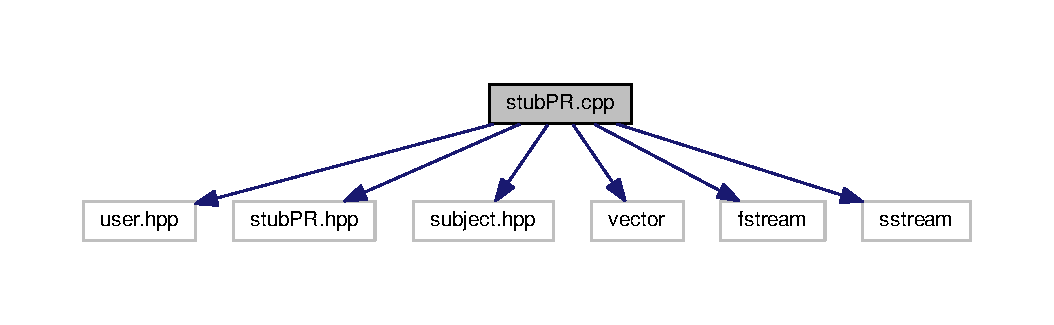
\includegraphics[width=350pt]{stubPR_8cpp__incl}
\end{center}
\end{figure}

\hypertarget{subject_8cpp}{}\section{subject.\+cpp File Reference}
\label{subject_8cpp}\index{subject.\+cpp@{subject.\+cpp}}
{\ttfamily \#include \char`\"{}subject.\+hpp\char`\"{}}\\*
{\ttfamily \#include $<$vector$>$}\\*
{\ttfamily \#include $<$string$>$}\\*
{\ttfamily \#include \char`\"{}helper.\+hpp\char`\"{}}\\*
{\ttfamily \#include \char`\"{}topic.\+hpp\char`\"{}}\\*
Include dependency graph for subject.\+cpp\+:
\nopagebreak
\begin{figure}[H]
\begin{center}
\leavevmode
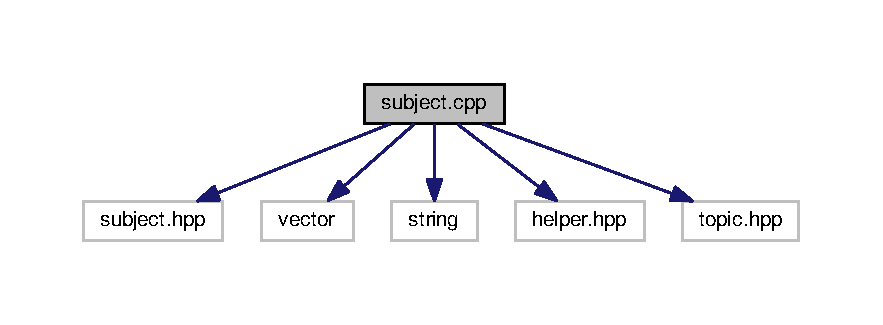
\includegraphics[width=350pt]{subject_8cpp__incl}
\end{center}
\end{figure}

\hypertarget{topic_8cpp}{}\section{topic.\+cpp File Reference}
\label{topic_8cpp}\index{topic.\+cpp@{topic.\+cpp}}
{\ttfamily \#include \char`\"{}topic.\+hpp\char`\"{}}\\*
{\ttfamily \#include $<$vector$>$}\\*
{\ttfamily \#include \char`\"{}helper.\+hpp\char`\"{}}\\*
{\ttfamily \#include \char`\"{}quiz.\+hpp\char`\"{}}\\*
Include dependency graph for topic.\+cpp\+:
\nopagebreak
\begin{figure}[H]
\begin{center}
\leavevmode
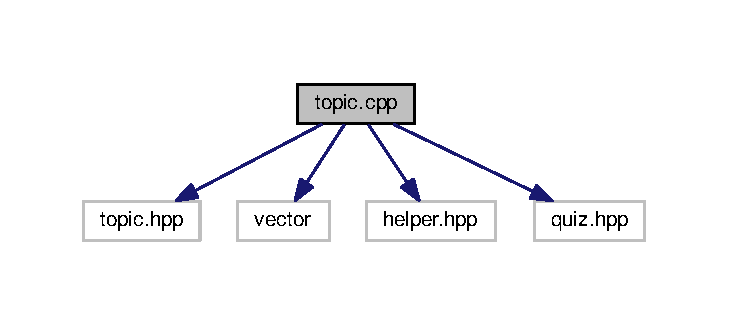
\includegraphics[width=350pt]{topic_8cpp__incl}
\end{center}
\end{figure}

\hypertarget{user_8cpp}{}\section{user.\+cpp File Reference}
\label{user_8cpp}\index{user.\+cpp@{user.\+cpp}}
{\ttfamily \#include \char`\"{}user.\+hpp\char`\"{}}\\*
{\ttfamily \#include $<$string$>$}\\*
{\ttfamily \#include $<$vector$>$}\\*
{\ttfamily \#include $<$algorithm$>$}\\*
{\ttfamily \#include \char`\"{}helper.\+hpp\char`\"{}}\\*
{\ttfamily \#include \char`\"{}subject.\+hpp\char`\"{}}\\*
{\ttfamily \#include \char`\"{}topic.\+hpp\char`\"{}}\\*
{\ttfamily \#include \char`\"{}quiz.\+hpp\char`\"{}}\\*
Include dependency graph for user.\+cpp\+:
\nopagebreak
\begin{figure}[H]
\begin{center}
\leavevmode
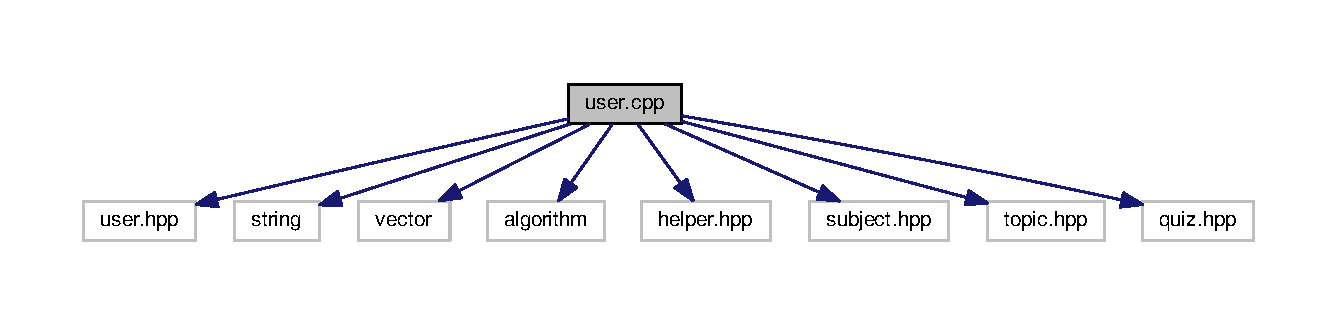
\includegraphics[width=350pt]{user_8cpp__incl}
\end{center}
\end{figure}

%--- End generated contents ---

% Index
\backmatter
\newpage
\phantomsection
\clearemptydoublepage
\addcontentsline{toc}{chapter}{Index}
\printindex

\end{document}
